\begin{slide}
\heading{Readers and writers}

The \emph{readers and writers problem} is a classic synchronisation problem.
Consider a collection of threads (or processes), each of which want to access
a database concurrently, some for reading and some for writing.  It is
allowable for several readers to be accessing the database simultaneously,
since their transactions will be independent.  However, it is not allowable
for two writers to have simultaneous access, nor for a reader and writer to
have simultaneous access.
\end{slide}

%%%%%


\begin{slide}
\heading{Readers and writers}

We will implement a controller object that controls access to the database,
implementing the following trait.
\begin{scala}
/** Trait for a readers and writers lock. */
trait ReadersWritersLock{
  def readerEnter: Unit
  def readerLeave: Unit
  def writerEnter: Unit
  def writerLeave: Unit
}
\end{scala}
%
The |Enter| methods will block, until the thread is allowed to use the
database. 
\end{slide}

%%%%%

\begin{slide}
\heading{Readers and writers}

The readers and writers call the appropriate operation before
and after  using the database; for example:
%
\begin{scala}
def reader(me: Int, rw: ReadersWritersLock) = thread{
  repeat{
    <operations not using database>
    rw.readerEnter // entry protocol
    <read the database>
    rw.readerLeave // exit protocol
  }
}
\end{scala}
\end{slide}

%%%%%

\begin{slide}
\heading{A simple implementation}

The |ReadersWritersLock| needs to keep track of the number of readers and
writers currently using the database, and maintain a suitable invariant.
%
\begin{scala}
class ReadersWritersMonitor extends ReadersWritersLock{
  private var readers = 0; private var writers = 0
  // Invariant: writers <= 1 && (readers == 0 || writers == 0)
  ...
}    
\end{scala}
\end{slide}

%%%%%

\begin{slide}
\heading{A simple implementation}

\begin{scala}
  def readerEnter = synchronized{
    while(writers > 0) wait()
    readers += 1
  }

  def readerLeave = synchronized{
    readers -= 1; notifyAll()
  }

  def writerEnter = synchronized{
    while(writers > 0 || readers > 0) wait()
    writers = 1
  }
      
  def writerLeave = synchronized{
    writers = 0; notifyAll()
  }
\end{scala}
\end{slide}


% \begin{slide}
% \heading{The controller}

% The controller needs to keep track of the number of readers and writers
% currently using the database, and maintain the following invariant:
% \begin{scala}
% readers==0 && writers<=1 || writers==0
% \end{scala}
% \end{slide}

% %%%%%

% \begin{slide}
% \heading{The controller}

% \begin{scala}
% object RWController{
%   private var readers = 0; private var writers = 0;
%   // Invariant readers==0 && writers<=1 || writers==0

%   def ReaderEnter = synchronized{
%     while(writers>0) wait();
%     readers+=1;
%   }

%   def WriterEnter = synchronized{
%     while(writers>0 || readers>0) wait();
%     writers=1;
%   }

%   ...
% }
% \end{scala}
% \end{slide}

% %%%%%

% \begin{slide}
% \heading{The controller}

% \begin{scala}
% object RWController{
%   ...

%   def ReaderLeave = synchronized{
%     readers-=1; notifyAll();
%   }
      
%   def WriterLeave = synchronized{
%     writers=0; notifyAll();
%   }
% }
% \end{scala}
% \end{slide}

%%%%%

\begin{slide}
\heading{Waking up}

Suppose a writer is currently accessing the database, and there are several
readers and writers waiting.  When the writer finishes and performs
|notifyAll|, all the waiting readers and writers become runnable.  One of
two things may occur:
%
\begin{itemize}
\item
A reader obtains the lock first, sets |readers = 1|, and accesses the database.
When the other writers are scheduled, they find \SCALA{readers > 0} and so
again \SCALA{wait}.  When the other readers are scheduled, they can also access
the database.

\item
A writer obtains the lock first, sets |writers = 1|, and accesses the
database.  When the other readers and writers are scheduled, they find
\SCALA{writers > 0} and so again \SCALA{wait}.
\end{itemize}
\end{slide}

%%%%%

\begin{slide}
\heading{Testing}

We can test the |ReadersWritersLock| by logging and then examining the log.
%
\begin{itemize}
\item Arrange for each thread to log entering and leaving the database
(for either reading or writing): logging entering should be done
\emph{after} entering, and logging leaving should be done
\emph{before} leaving:%
%
\begin{scala}
  rw.readerEnter; log.add(me, ReaderEnter)
  ...
  log.add(me, ReaderLeave); rw.readerLeave
\end{scala}
This ensures that the period between the log events is a subset of the period
when the thread is allowed to use the database, to avoid false positives.
      
\item When all threads have finished, traverse the log to ensure the invariant
was maintained.

\item Repeat many times.
\end{itemize}
%
%See the code on the website.
\end{slide}

%%%%%

\begin{slide}
\heading{Starvation}

The previous version of the readers-writers lock was unfair.  

Consider a scenario where readers repeatedly enter and leave the database, and
such that there is always at least one reader using it (even though no single
reader remains in the database).  The writers are starved!
\begin{center}
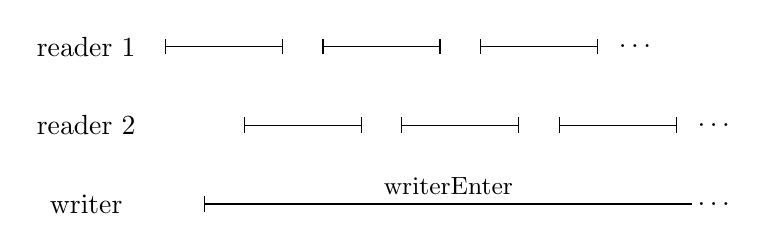
\begin{tikzpicture}
\draw (0,0) node{reader 1};
\draw[|-|] (1,0) -- (2.5,0); \draw[|-|] (3.0,0) -- (4.5,0); 
\draw[|-|] (5.0,0) -- (6.5,0); \draw (7.0,0) node{\ldots};
\draw (0,-1) node{reader 2}; 
\draw[|-|] (2.0,-1) -- (3.5,-1); \draw[|-|] (4.0,-1) -- (5.5,-1); 
\draw[|-|] (6.0,-1) -- (7.5,-1); \draw (8.0,-1) node{\ldots};
\draw (0,-2) node{writer}; 
\draw[|-] (1.5,-2) -- node[above]{\small\scalashape writerEnter} (7.7,-2);
\draw (8.0,-2) node{\ldots};
\end{tikzpicture}
\end{center}
\end{slide}

%%%%%

\begin{slide}
\heading{Avoiding starvation}

We give a fair version, using the following idea:
%
\begin{itemize}
\item Each writer registers its interest before actually entering the
database;

\item If a writer has registered its interest, no reader subsequently enters.
\end{itemize}
%
Thus eventually all the current readers will leave, and the writer can enter. 
\end{slide}

%%%%%

\begin{slide}
\heading{A fair readers-writers lock}

\begin{scala}
class FairReadWriteLock extends ReadersWritersLock{
  private var readers = 0 // current # readers in the CS
  private var writers = 0 // current # writers in the CS or trying

  def readerEnter = synchronized{
    while(writers > 0) wait() // wait for writer to leave
    readers += 1 // record my entry
  }

  def readerLeave = synchronized{
    readers -= 1 // record my exit
    if(readers == 0) notifyAll() // signal to waiting writer
  }
  ...
}
\end{scala}
\end{slide}

%%%%%

\begin{slide}
\heading{A fair readers-writers lock}

\begin{scala}
  def writerEnter = synchronized{
    while(writers > 0) wait() // wait until no writer ahead of me
    writers = 1 // record that I'm trying; readers are blocked
    while(readers > 0) wait() // wait for readers to leave
  }

  def writerLeave = synchronized{
    writers = 0 // record my exit
    notifyAll() // signal to waiting reader or writer
  }
\end{scala}

This avoids starvation provided the JVM monitor is fair.
\end{slide}

